\subsection{Methane pyrolysis in shock-tube using constant pressure reactor}
The pyrolysis of 5\% and 10\% $\mathrm{CH_4}$-Ar was investigated using a constant pressure reactor model (CPR) for the post-shock temperature, $T_5$ range of 1800-3000 K, and pressure, $\mathrm{P_5}$ range of 4.7-7.1 bar. $P_5$ was not specified for each experiment (characterized with $\mathrm{T_5}$), so we assume that $P_5$ linearly increases with $\mathrm{T_5}$. Caltech mechanism was used to describe gas chemistry. The inception and PAH adsorption rates were adjusted using $\eta_{inc}$ and $\eta_{ads}$, respectively to match the predicted carbon yield at t=1.5 ms over the studied $\mathrm{T_5}$ and $\mathrm{P_5}$ with the extinction measurements at $\mathrm{\lambda}$=632~nm~\citep{agafonov2016unified}.The measured carbon yield was retrieved from the reported yield$\times$E(m) considering the maximum variability in the absorption function of soot from 0.174~\citep{lee1981optical} to 0.37~\citep{agafonov2011soot} in the literature. Both adjustment factors were varied between 0 and 1, ad Our parametric studies showed that there is not a


\begin{figure}[H]
	\centering
	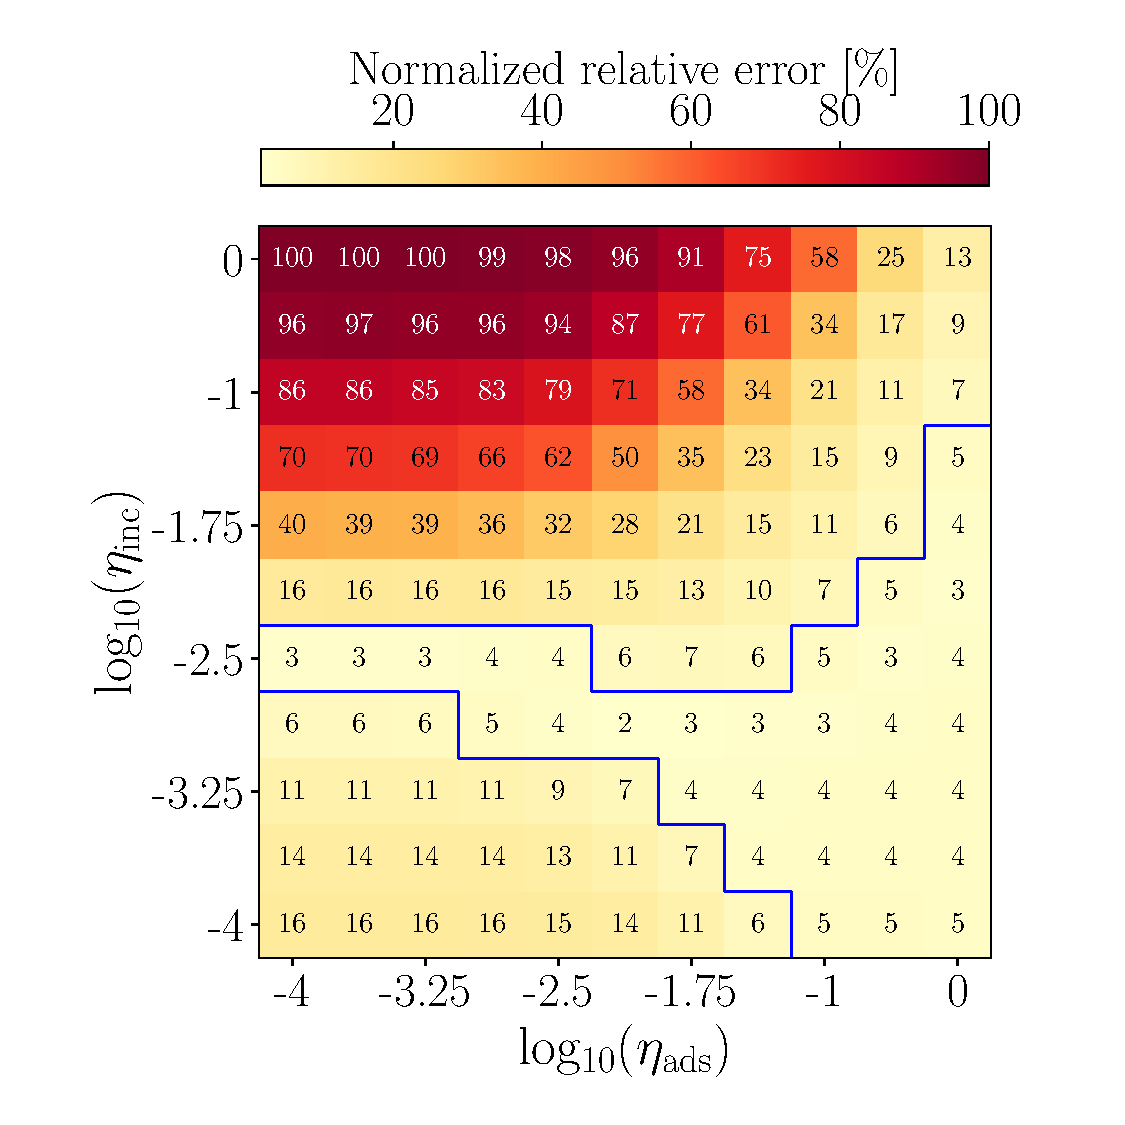
\includegraphics[width=0.5\textwidth]{Figures/Results/Shocktube/Agafonov2016_cpr/5CH4_norm_yield_error_readim.pdf}
	\caption{The relative error of carbon yield normalized by the maximum value at t=1.5 ms for 5\%~$\mathrm{CH_4}$ obtained using Caltech mechanism and Reactive Dimerization}.
	\label{fig:shockagof_yielderror_cpr} 
\end{figure}


First, the model was run without soot (only the gas phase is simulated and no soot conversion allowed) to provide insight into the effect of temperature on the species involved in soot formation. Fig.~\ref{fig:SPC_cmf}-a shows the carbon mass fraction (CMF) of soot precursors at 1.5 ms that exhibits a bell-shape behavior reaching 7 and 12\% of total carbon mass for 5 and 10\% $\mathrm{CH_4}$, respectively. The temperature of the peak CMF is 2350 K for 10\% $\mathrm{CH_4}$ higher than that of 5\% $\mathrm{CH_4}$ 2125 K. On the other hand, the CMF of $\mathrm{C_2H_2}$ at 1.5 ms, shown in Fig.~\ref{fig:SPC_cmf_cpr}-b, increases linearly with temperature and then levels off. While doubling the initial $\mathrm{CH_4}$ mole fraction increases the peak CMF of precursors by nearly a factor of two, the maximum CMF of $\mathrm{C_2H_2}$ is nearly 0.85 for both cases.

\begin{figure}[H]
	\centering
	\begin{subfigure}[t]{0.4\textwidth}
		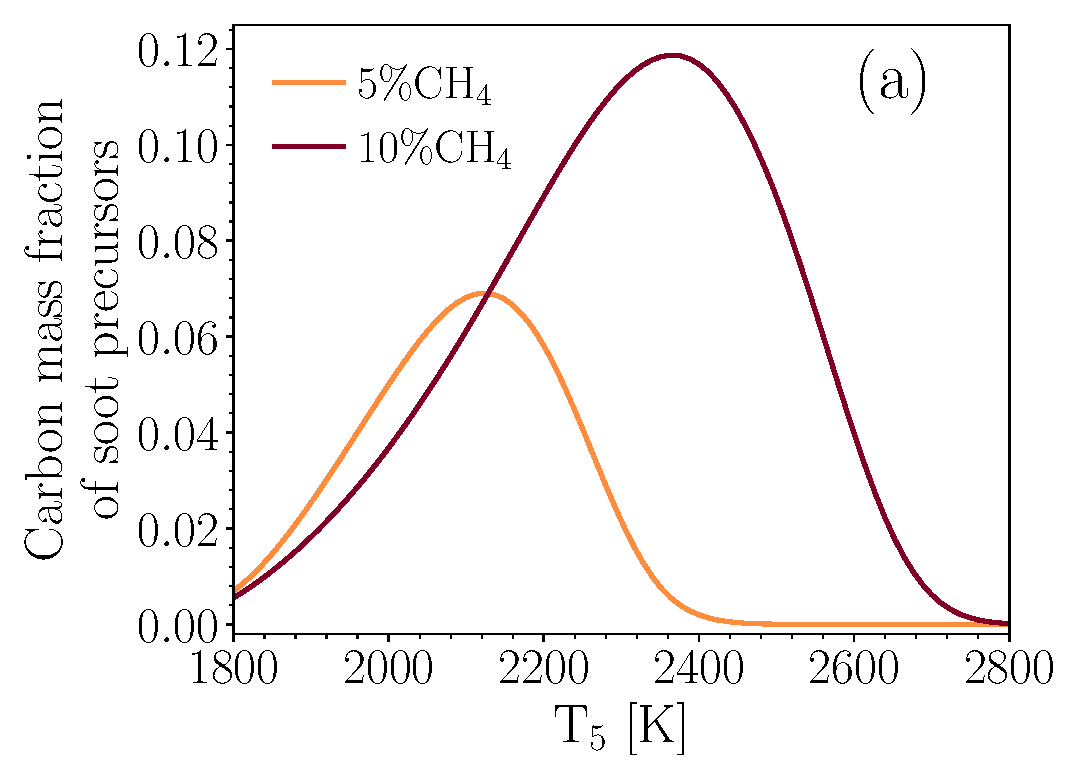
\includegraphics[width=1\textwidth]{Figures/Results/Shocktube/Agafonov2016_cpr/SPC_cmf.pdf}
	\end{subfigure}
	\begin{subfigure}[t]{0.36\textwidth}
		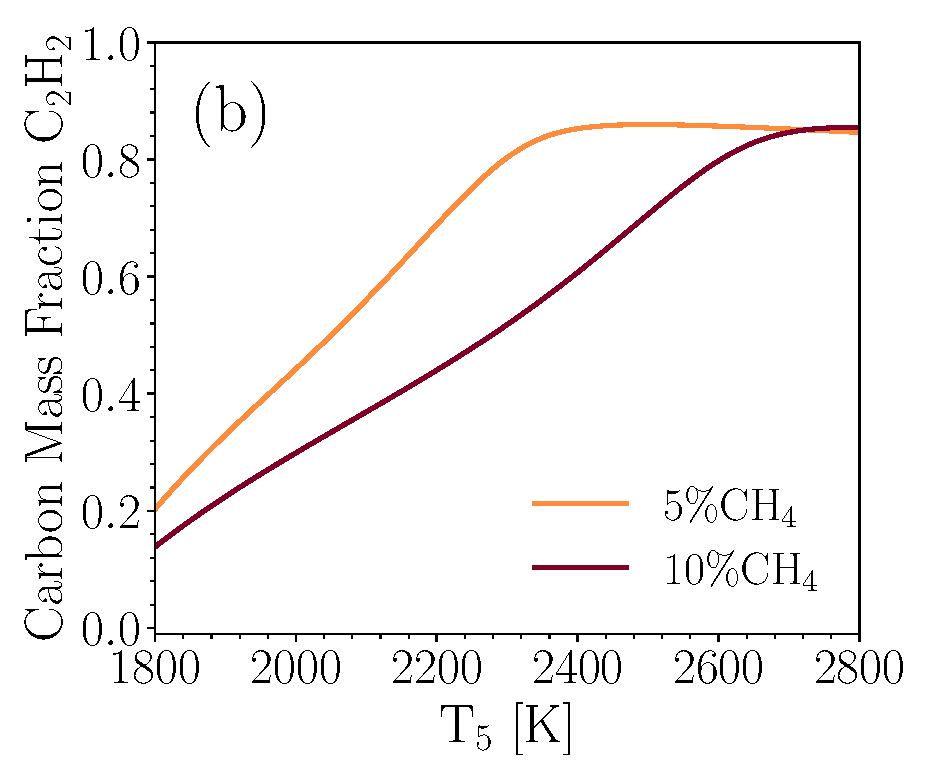
\includegraphics[width=1\textwidth]{Figures/Results/Shocktube/Agafonov2016_cpr/C2H2_cmf.pdf}
	\end{subfigure}
	\caption{The bell-shape temperature profile of carbon mass fraction of soot precursors (A2 and larger) combined (a) and $\mathrm{C_2H_2}$ (b) at t=1.5 ms during pyrolysis of 5\% (red line) and 10\%~$\mathrm{CH_4}$-Ar (green line) obtained using CPR model with Caltech mechanism without considering soot}
	\label{fig:SPC_cmf_cpr} 
\end{figure}

Next set of simulations were conducted by using equal adjustment factor ($\eta_{inc}=\eta_{ads}$) to minimize prediction error of mean soot carbon yield
Fig.~\ref{fig:shockagof_yield_cpr} compares soot carbon yield predicted using the different inception models and the sectional population balance model with the data from extinction measurements~\citep{agafonov2016unified}. A skew exponential curve (represented by the black dotted line) was fitted to the data to highlight the trend in carbon yield, and its likely peak, which increases with initial methane mole fraction from 12 to 32\%. Soot carbon yield has a bell-shape profile similar to the one shown for soot precursor because soot inception flux and mass growth are directly tied to the concentration of precursors. All the inception models capture of the expected trend. As shown in Fig.~\ref{fig:shockagof_yield_cpr}-a, the agreement between the predicted carbon yield and the measurements are better for \%5 $\mathrm{CH_4}$ especially in $\mathrm{T_5}$<2400 K. The yield predicted by Reactive Dimerization at $\mathrm{T_5}$ less than the temperature of the peak yield is slightly larger than the other inception models. EBridge Modified seems to shifted to higher temperatures compared to other inception models indicating different temperature dependence of this model (PAH dehydrogenation) is described with an Arrhenius rate as opposed to the other model where inception is initiated with physical collision of PAHs.

\begin{figure}[H]
	\centering
	\begin{tikzpicture}
		\draw (0, 0) node[inner sep=0] 	{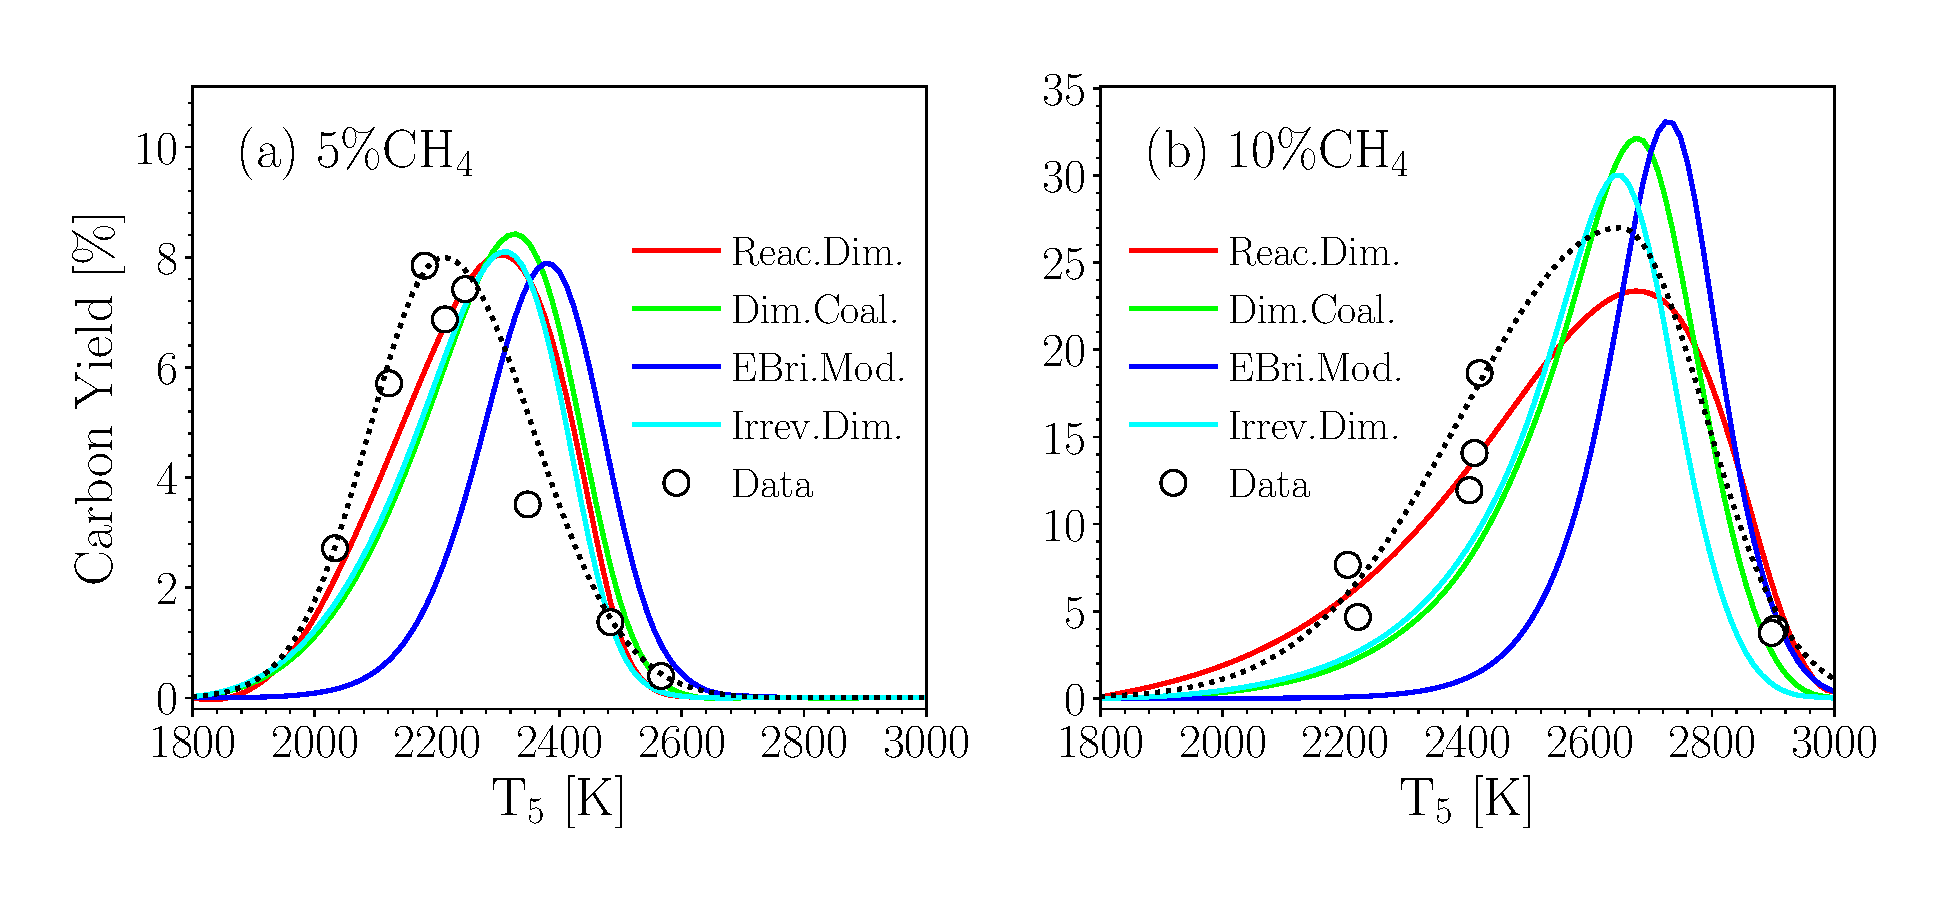
\includegraphics[width=0.8\textwidth]{Figures/Results/Shocktube/Agafonov2016_cpr/carbon_yield.pdf}};
		\draw (-0.52, -0.02) node {\scriptsize{\cite{agafonov2016unified}}};
		%\draw (2.42, -0.23) node {\scriptsize{\cite{agafonov2016unified}}};
	\end{tikzpicture}
	\caption{The bell-shape temperature profile of soot carbon yield at t=1.5 ms for 5\% (a) and 10\%~$\mathrm{CH_4}$ (b) in Ar obtained using Caltech mechanism and different inception models calibrated to minimize the prediction with extinction measurements~\citep{agafonov2016unified}. The dashed line was added to show the trend in the measurements.}
	\label{fig:shockagof_yield_cpr} 
\end{figure}


As shown in Fig.\ref{fig:shockagof_dp_cpr}, the predicted $d_p$ increases with $\mathrm{T_5}$ over the studied temperature range. The differences between inception models is overall negligible except for Reactive Dimerization, which predicts a larger $d_p$ compared to other inception models in $\mathrm{T_5}$ range lower than 2500 and 2700 K for 5\% and 10\% $\mathrm{CH_4}$, respectively. As shown in Eq.\eqref{eqn:d_p}, $d_p$ is proportional of the third-root of $C_{tot}/N_{pri}$. $C_{tot}$ describes total carbon mass converted to soot through inception and surface growth while $N_{pri}$ is only determined by inception flux. As a result, $d_p$ is controlled by the ratio of surface growth (HACA and PAH adsorption) rate to inception flux. To better understand this, the ratio of carbon mass gained by each pathway to the total soot carbon mass at 1.5 ms is calculated and shown in Fig.\ref{fig:shockagof_carbon_map_cpr}. In the low temperature range, $\mathrm{T_5}<$2000 K, Reactive Dimerization directs the majority of the converted carbon to HACA and PAH adsorption (see Fig.\ref{fig:shockagof_carbon_map_cpr}-a,b) resulting in larger $C_{tot}/N_{pri}$ compared to other inception models that corresponds to larger $d_p$ values. The carbon mass fraction of inception decreases with temperature for all inception models leading to increasing $d_p$.

\begin{figure}[H]
	\centering
	\includegraphics[width=0.8\textwidth]{Figures/Results/Shocktube/Agafonov2016_cpr/d_p.pdf}
	\caption{The temperature dependence of mean primary particle diameter, $d_p$ at t=1.5 ms for 5\% (a) and 10\%~$\mathrm{CH_4}$ (b) in Ar obtained using Caltech mechanism and different inception models calibrated to minimize the prediction with extinction measurements~\citep{agafonov2016unified}.}
	\label{fig:shockagof_dp_cpr} 
\end{figure}


\begin{figure}[H]
	\centering
	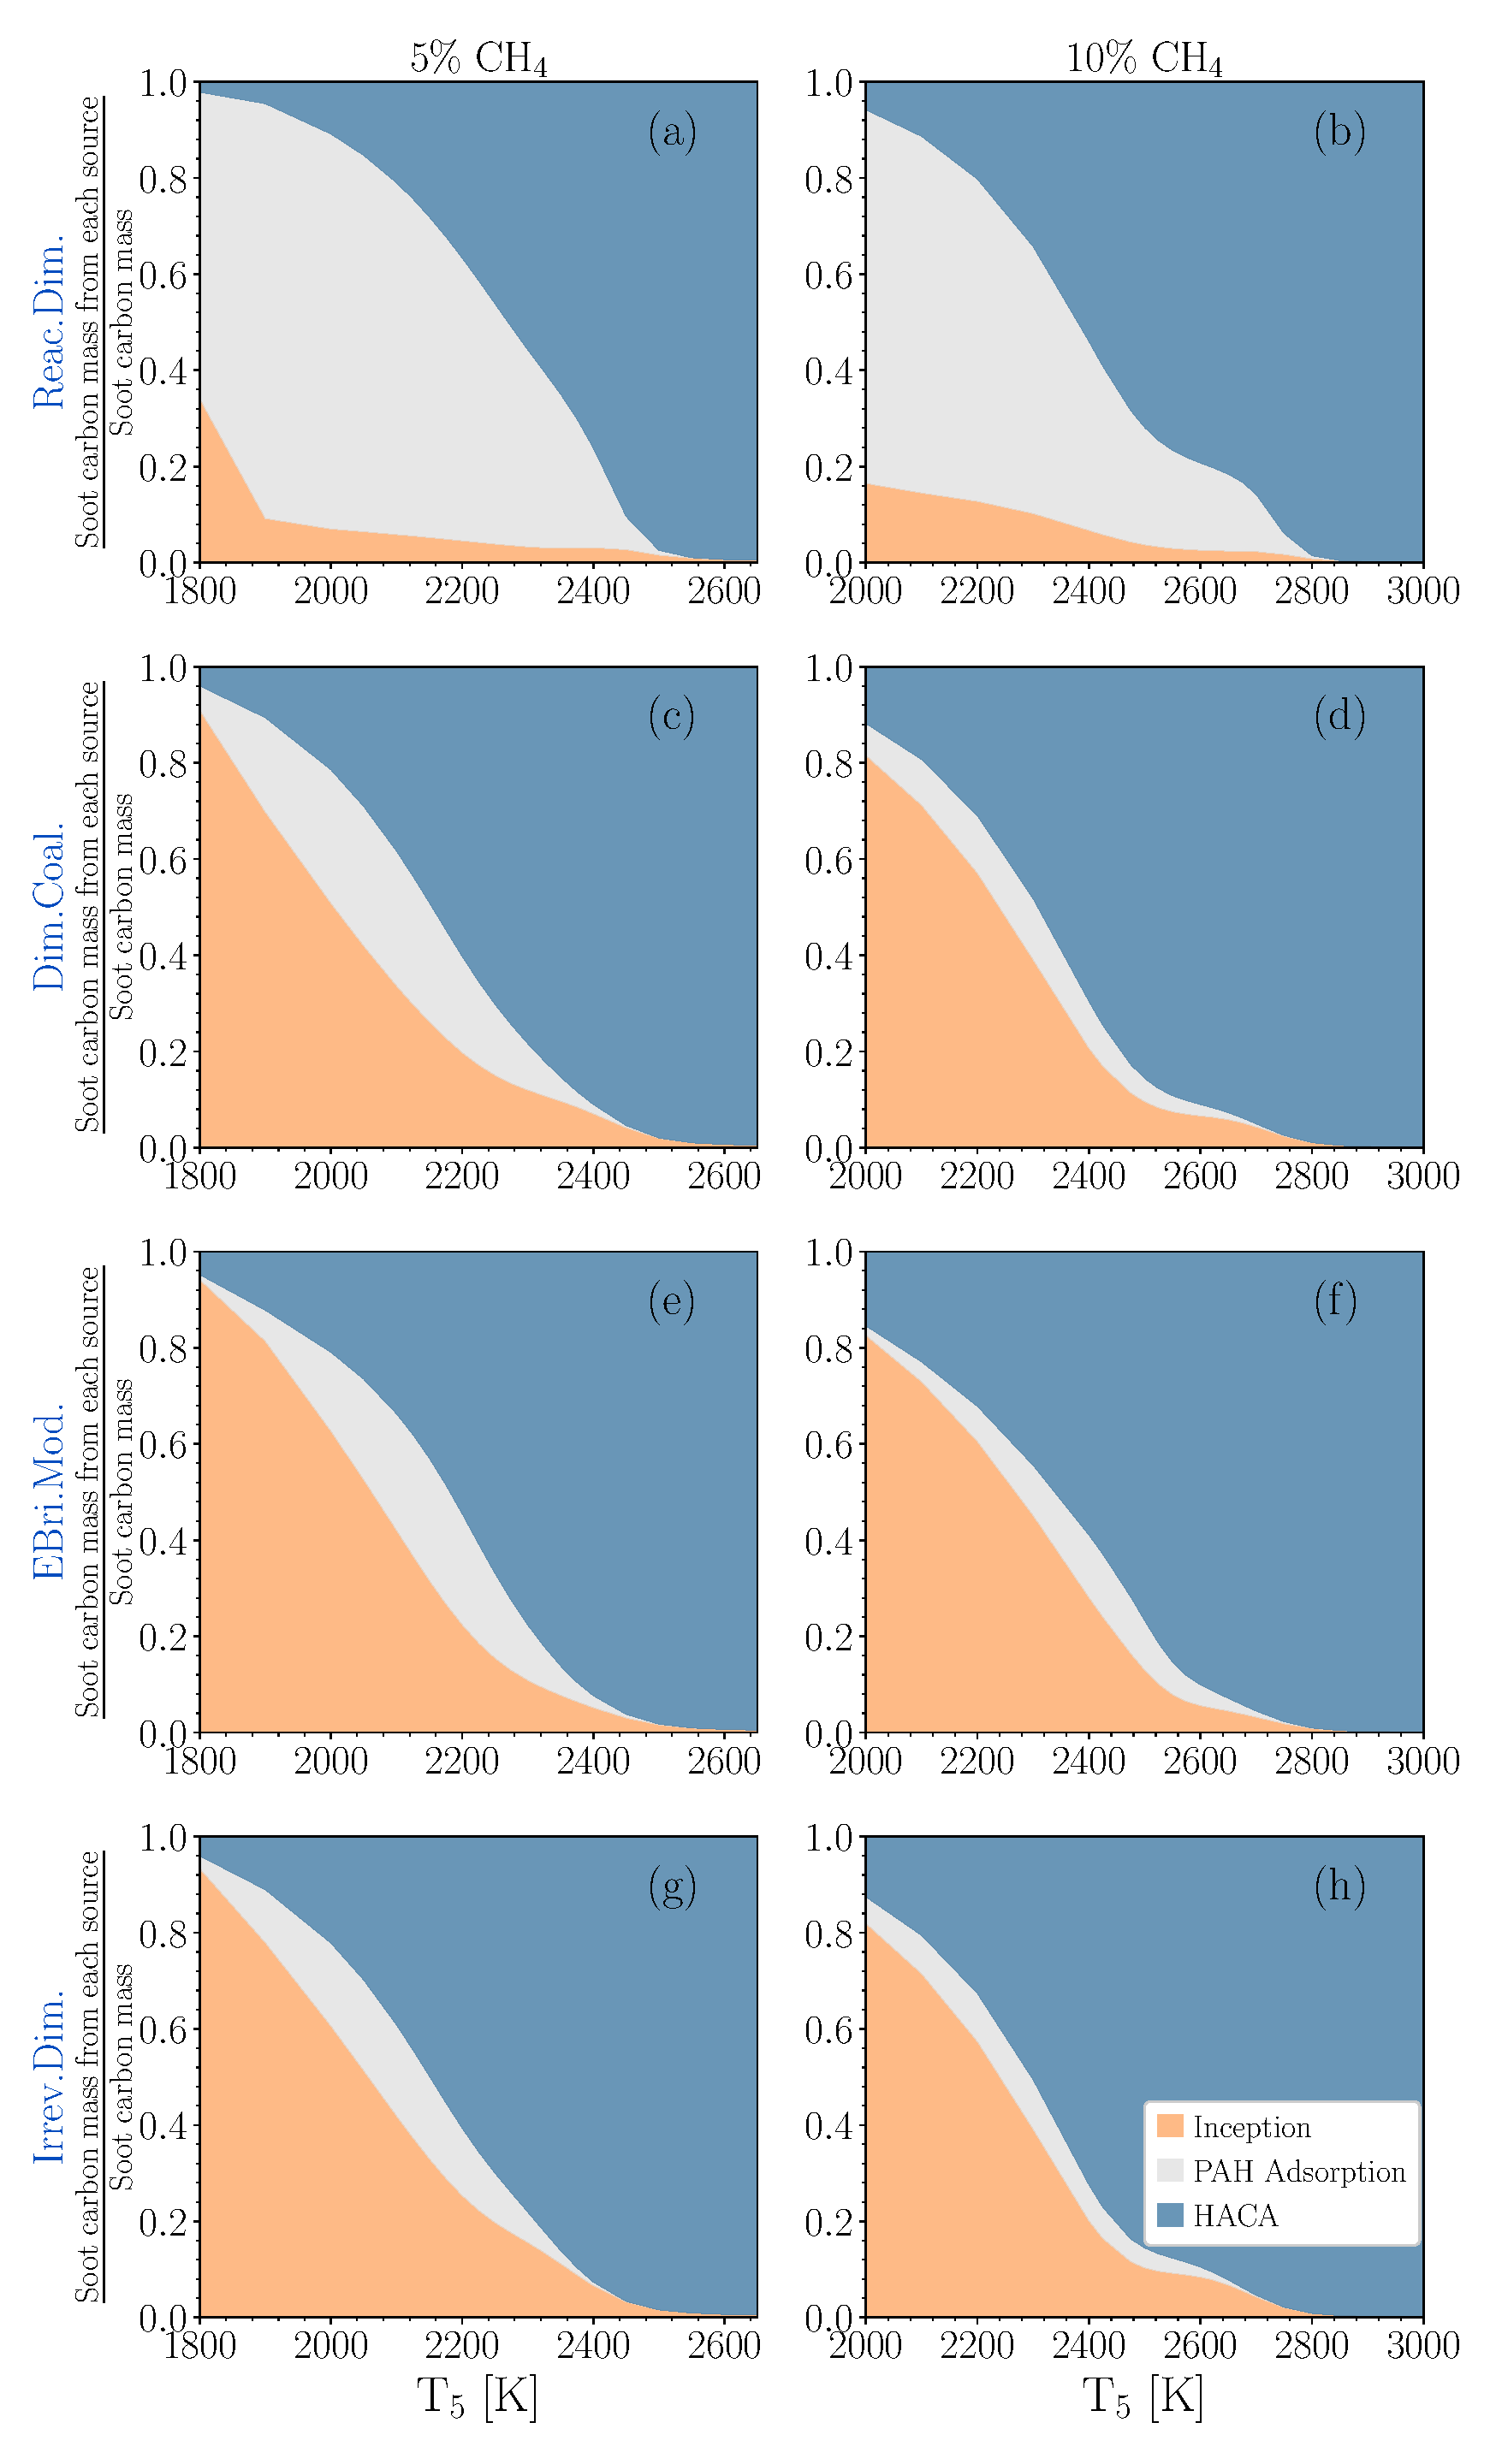
\includegraphics[width=0.8\textwidth]{Figures/Results/Shocktube/Agafonov2016_cpr/C_tot_distmap.pdf}
	\caption{The soot carbon mass from inception, PAH adsorption and HACA normalized by total soot carbon mass at t=1.5 ms for 5\% (a) and 10\%~$\mathrm{CH_4}$ (b) in Ar obtained using Caltech mechanism and different inception models calibrated to minimize the prediction with extinction measurements~\citep{agafonov2016unified}.}
	\label{fig:shockagof_carbon_map_cpr} 
\end{figure}

\begin{figure}[H]
	\centering
	\begin{tikzpicture}
		\draw (0, 0) node[inner sep=0] 	{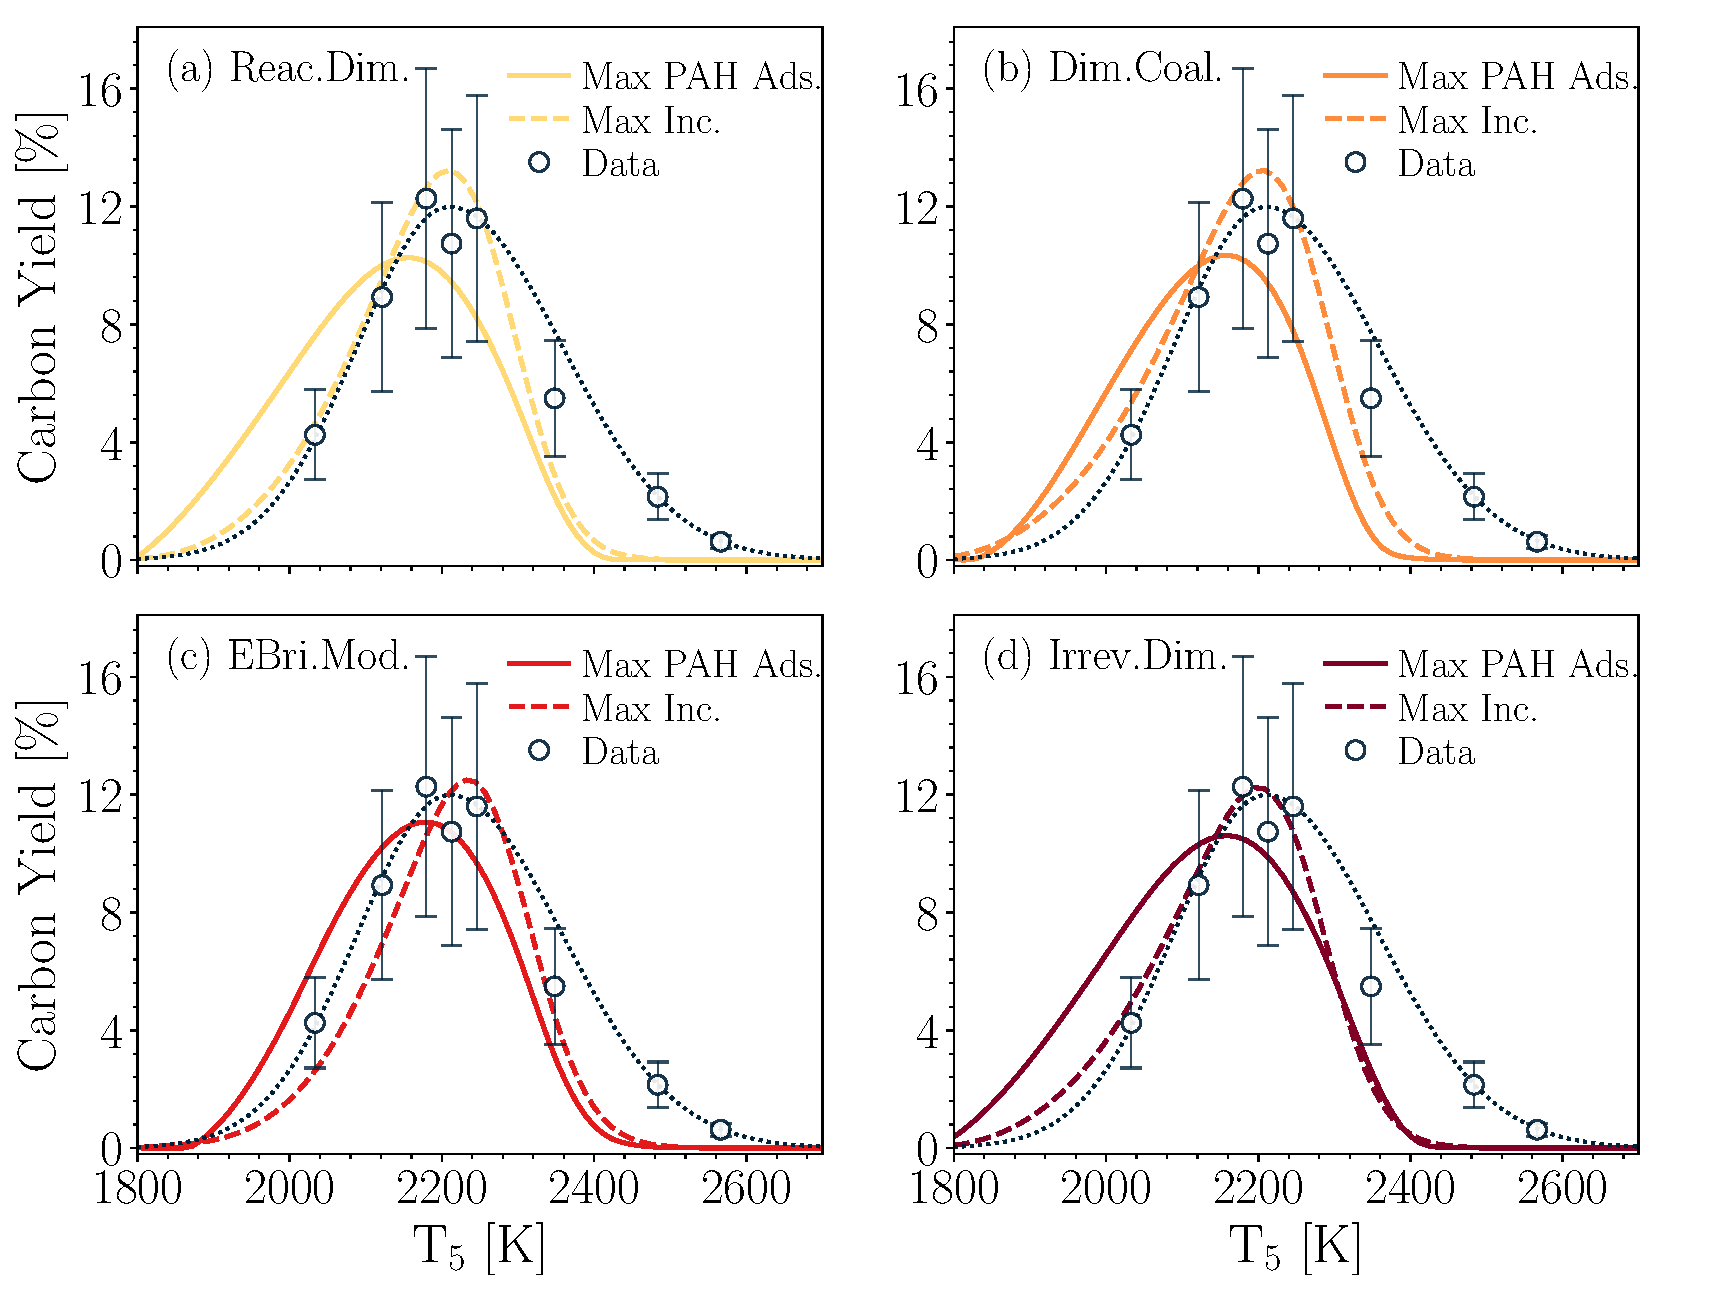
\includegraphics[width=0.8\textwidth]{Figures/Results/Shocktube/Agafonov2016_cpr/carbon_yield_maxincads.pdf}};
		\draw (-1.06, -0.78) node {\scriptsize{\cite{agafonov2016unified}}};
		\draw (4.75, -0.78) node {\scriptsize{\cite{agafonov2016unified}}};
		\draw (-1.06, 3.4) node {\scriptsize{\cite{agafonov2016unified}}};
		\draw (4.75, 3.4) node {\scriptsize{\cite{agafonov2016unified}}};
	\end{tikzpicture}
	\caption{The comparison of soot carbon yield at t=1.5 ms when maximum inception (dashed line) and PAH adsorption (solid line) were applied to minimized the prediction error compared to measurements~\citep{agafonov2016unified} for 5\% (a) and 10\%~$\mathrm{CH_4}$ (b) in Ar obtained using Caltech mechanism and different inception models.}
	\label{fig:shockagof_yield_maxincads_cpr} 
\end{figure}

\begin{figure}[H]
	\centering
	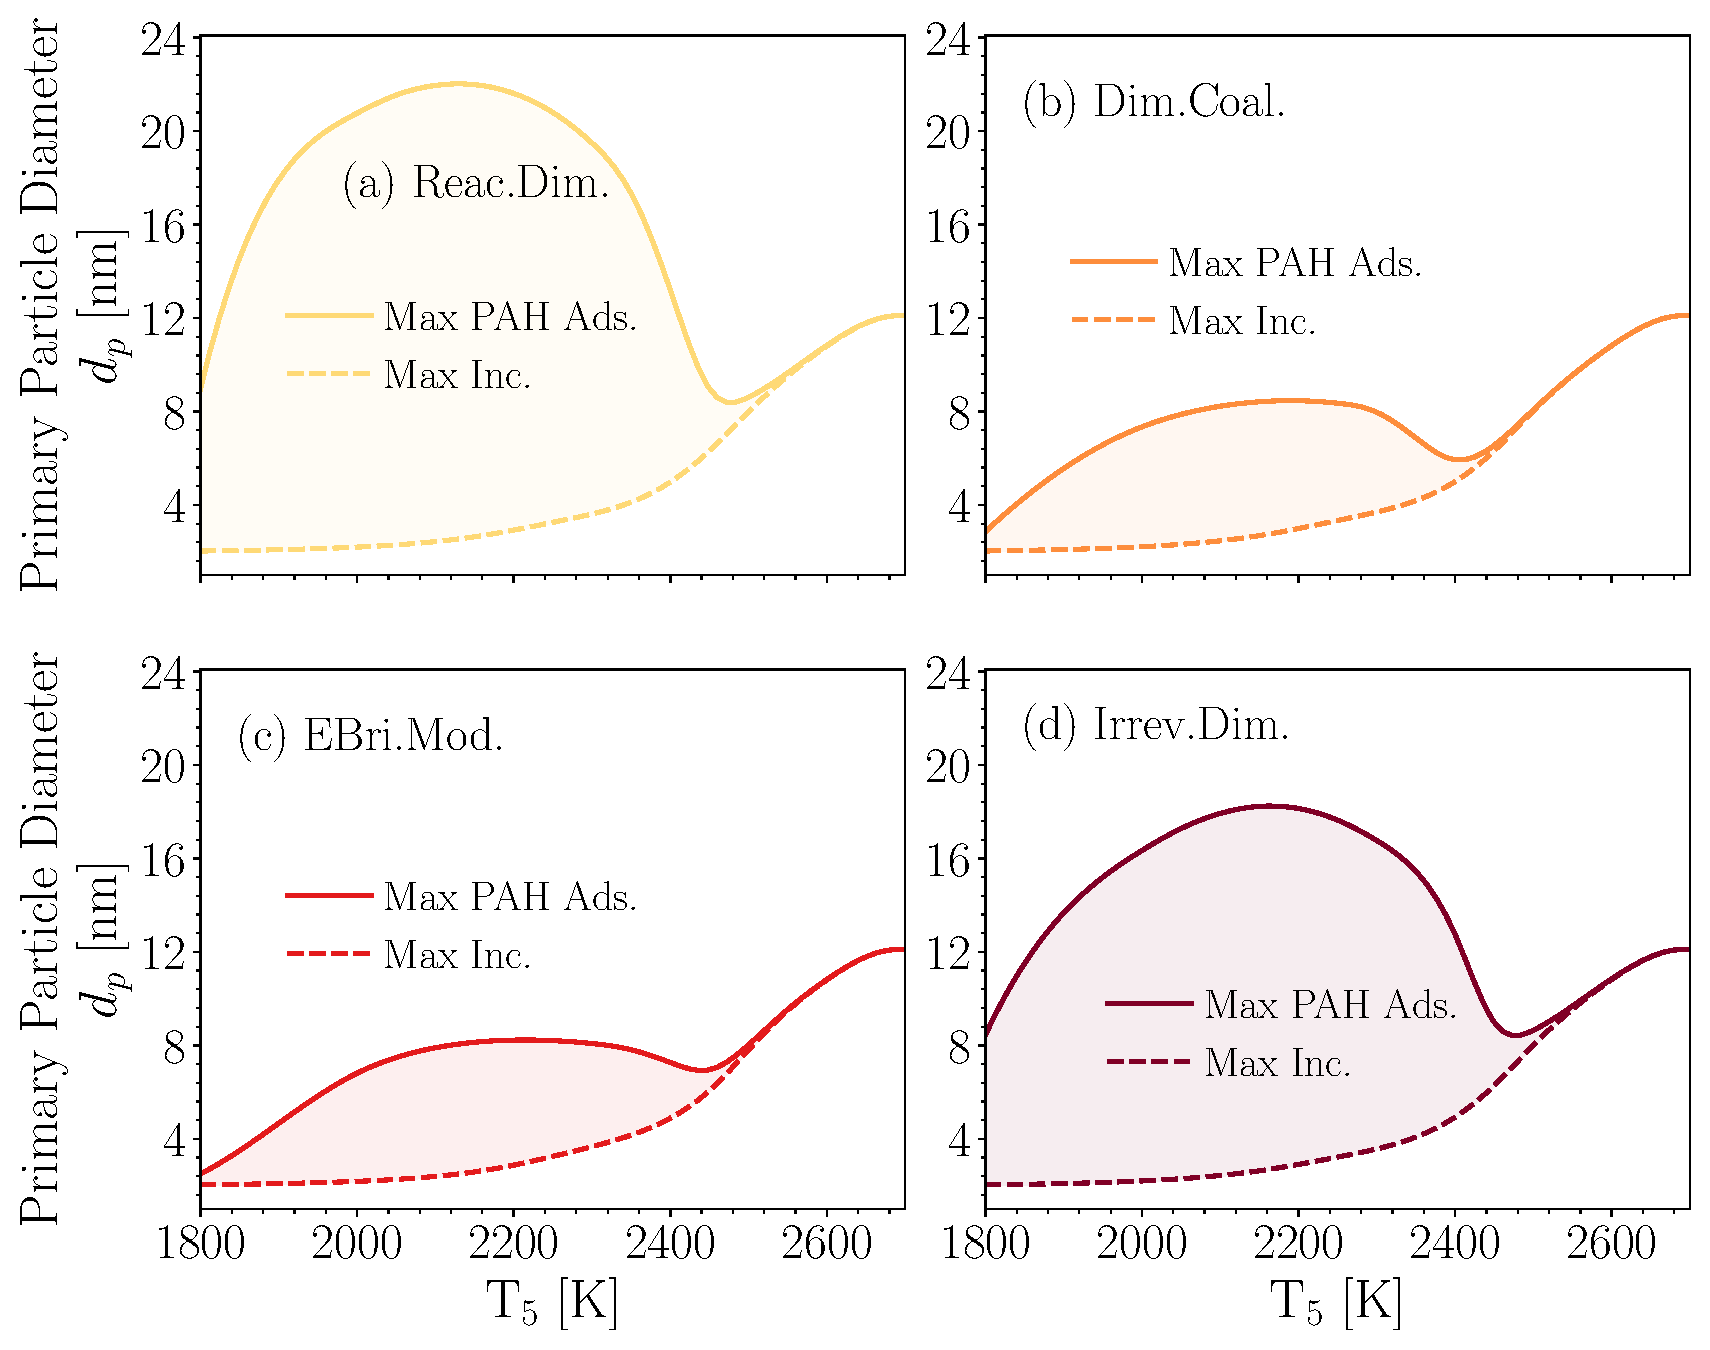
\includegraphics[width=0.8\textwidth]{Figures/Results/Shocktube/Agafonov2016_cpr/d_p_maxincads.pdf}
	\caption{The comparison of mean primary particle, $d_p$ at t=1.5 ms when maximum inception and PAH adsorption were applied to minimized the prediction  error compared to measurements~\citep{agafonov2016unified} for 5\% (a) and 10\%~$\mathrm{CH_4}$ (b) in Ar obtained using Caltech mechanism and different inception models.}
	\label{fig:shockagof_dp_maxincads_cpr} 
\end{figure}

\subsection{Methane pyrolysis in shock-tube using constant volume reactor}

%The pyrolysis of 5\% and 10\% $\mathrm{CH_4}$-Ar was investigated using a constant volume reactor model (CVR) for the post-shock temperature, $T_5$ range of 1800-3000 K, and pressure, $P_5$ range of 4.7-7.1 bar. $P_5$ was assumed to linearly increase with $T_5$ across the simulation cases. Caltech mechanism was used and the inception models were calibrated in order to match carbon yield at t=1.5 ms with the measurement~\citep{agafonov2016unified} using a dual-beam absorption–emission technique. \citet{agafonov2016unified} reported yield$\times$E(m) at $\mathrm{\lambda}$=632~nm, and yield data was retrieved using E(m)=0.37 suggested therein. 


\begin{figure}[H]
	\centering
	\begin{subfigure}[t]{0.4\textwidth}
		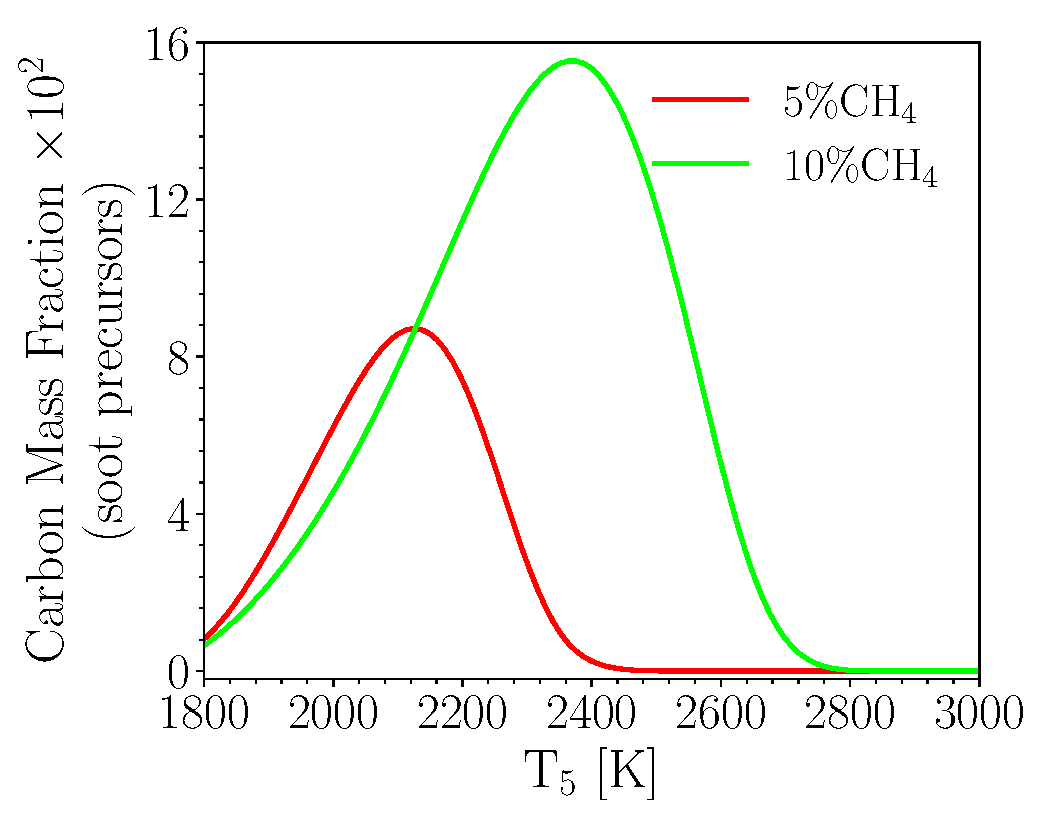
\includegraphics[width=1\textwidth]{Figures/Results/Shocktube/Agafonov2016_cvr/SPC_cmf.pdf}
	\end{subfigure}
	\begin{subfigure}[t]{0.4\textwidth}
		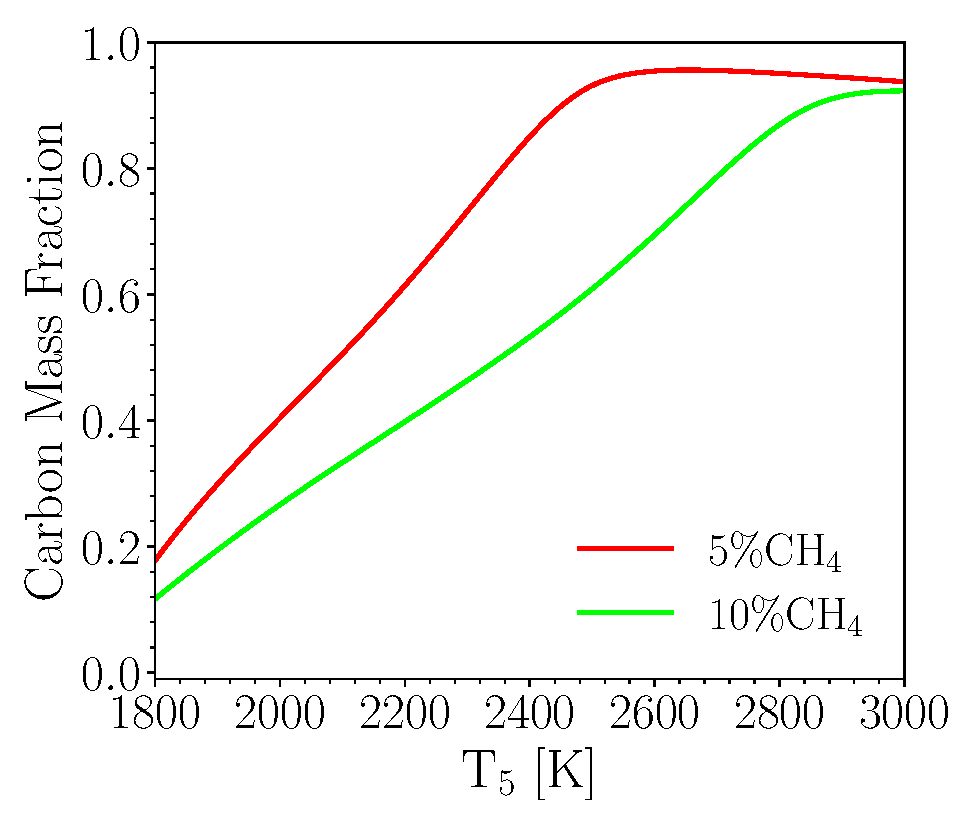
\includegraphics[width=1\textwidth]{Figures/Results/Shocktube/Agafonov2016_cvr/C2H2_cmf.pdf}
	\end{subfigure}
	\caption{The bell-shape temperature profile of carbon mass fraction of soot precursors (A2 and larger) combined (a) and $\mathrm{C_2H_2}$ (b) at t=1.5 ms during pyrolysis of 5\% (red line) and 10\%~$\mathrm{CH_4}$-Ar (green line) obtained using Caltech mechanism without considering soot}
	\label{fig:SPC_cmf_cvr} 
\end{figure}




\begin{figure}[H]
	\centering
	\begin{tikzpicture}
		\draw (0, 0) node[inner sep=0] 	{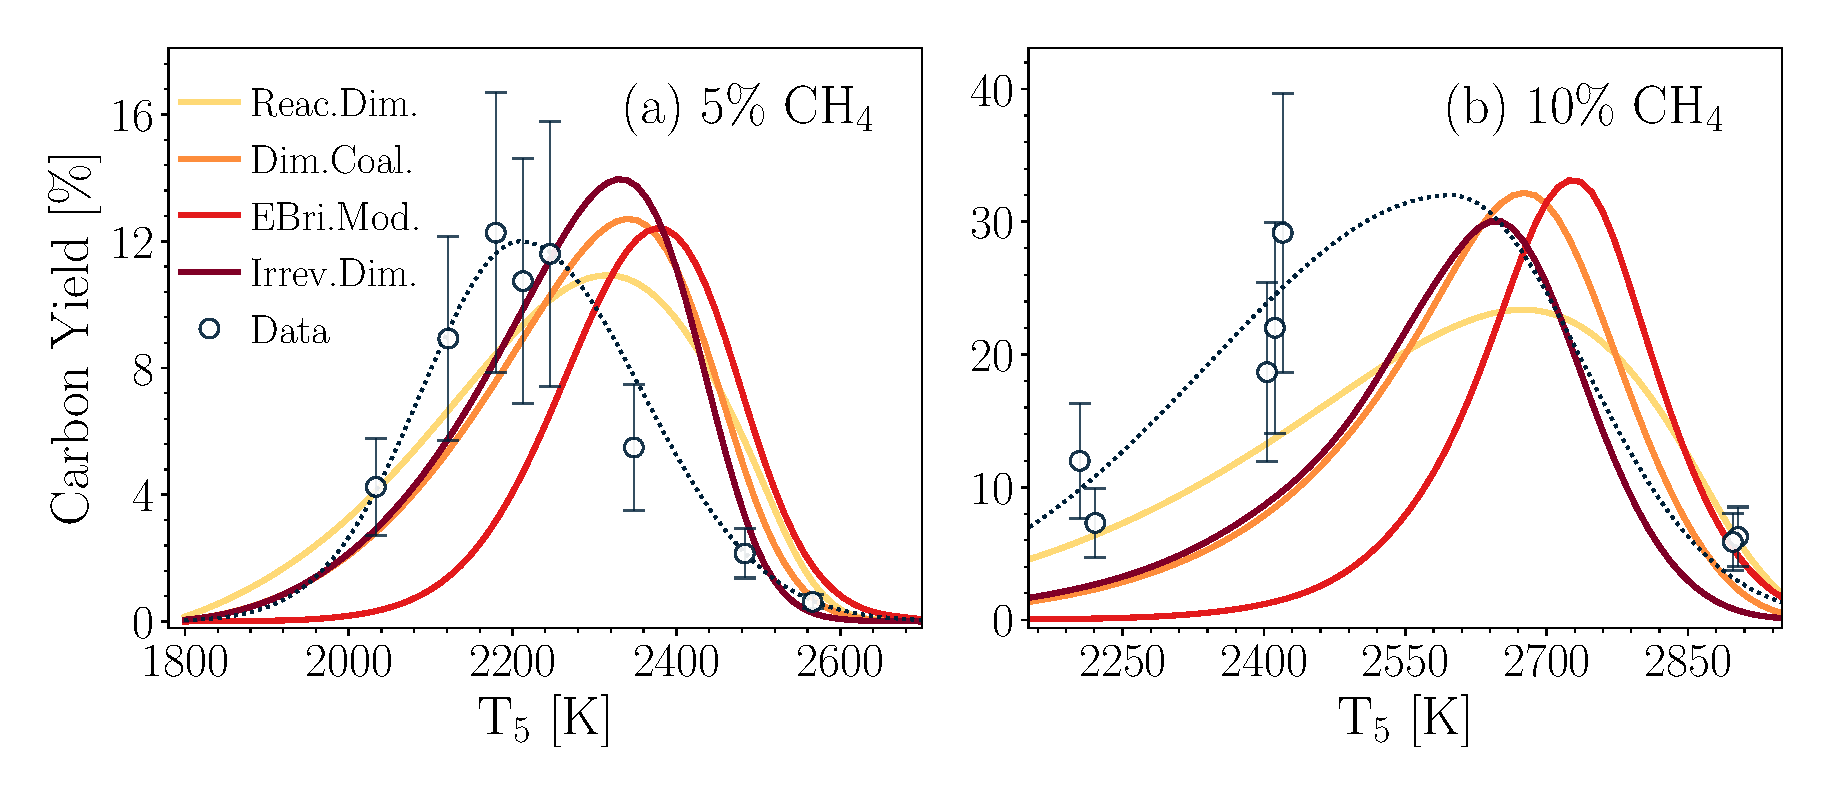
\includegraphics[width=0.8\textwidth]{Figures/Results/Shocktube/Agafonov2016_cvr/carbon_yield.pdf}};
		\draw (-3.6, 0.42) node {\scriptsize{\cite{agafonov2016unified}}};
		%\draw (2.42, -0.23) node {\scriptsize{\cite{agafonov2016unified}}};
	\end{tikzpicture}
	\caption{The bell-shape temperature profile of soot carbon yield at t=1.5 ms for 5\% (a) and 10\%~$\mathrm{CH_4}$ (b) in Ar obtained using Caltech mechanism and different inception models calibrated to minimize the prediction with extinction measurements~\citep{agafonov2016unified}.}
	\label{fig:shockagof_yield_cvr} 
\end{figure}

Fig.~\ref{fig:shockagof_yield} shows soot carbon yield predicted using Caltech mechanism where inception flux and PAH adsorption rate were adjusted using a scaling factor (equal for the both) to minimize the prediction error compared to the data from extinction measurements~\citep{agafonov2016unified}. A skew exponential curve fit (represented by the black dotted line) was applied to illustrate the trend in soot yield and identify the temperature at which the yield likely reaches its maximum. The predicted temperature of peak yield is larger than peak of curve-fit in both $\mathrm{CH_4}$ concentrations by 100-200 K depending on the inception model. This difference is due the contribution of  HACA to surface growth that depends on $\mathrm{C_2H_2}$ concentration which increases with temperature.

\begin{figure}[H]
	\centering
	\includegraphics[width=0.8\textwidth]{Figures/Results/Shocktube/Agafonov2016_cvr/d_p.pdf}
	\caption{The temperature dependence of mean primary particle diameter, $d_p$ at t=1.5 ms for 5\% (a) and 10\%~$\mathrm{CH_4}$ (b) in Ar obtained using Caltech mechanism and different inception models calibrated to minimize the prediction with extinction measurements~\citep{agafonov2016unified}.}
	\label{fig:shockagof_dp_cvr} 
\end{figure}

Fig.\ref{fig:shockagof_dp} shows that $d_p$ increases with temperature up to 10 nm. For 5\% $\mathrm{CH_4}$, $d_p$ reaches the peak around 2800 K and drops quickly to 2 nm which is the minimum allowed diameter in the model. Reactive Dimerization results in overall larger primary particle diameters, but the behavior of the rest of inception models are similar.

\begin{figure}[H]
	\centering
	\begin{tikzpicture}
		\draw (0, 0) node[inner sep=0] 	{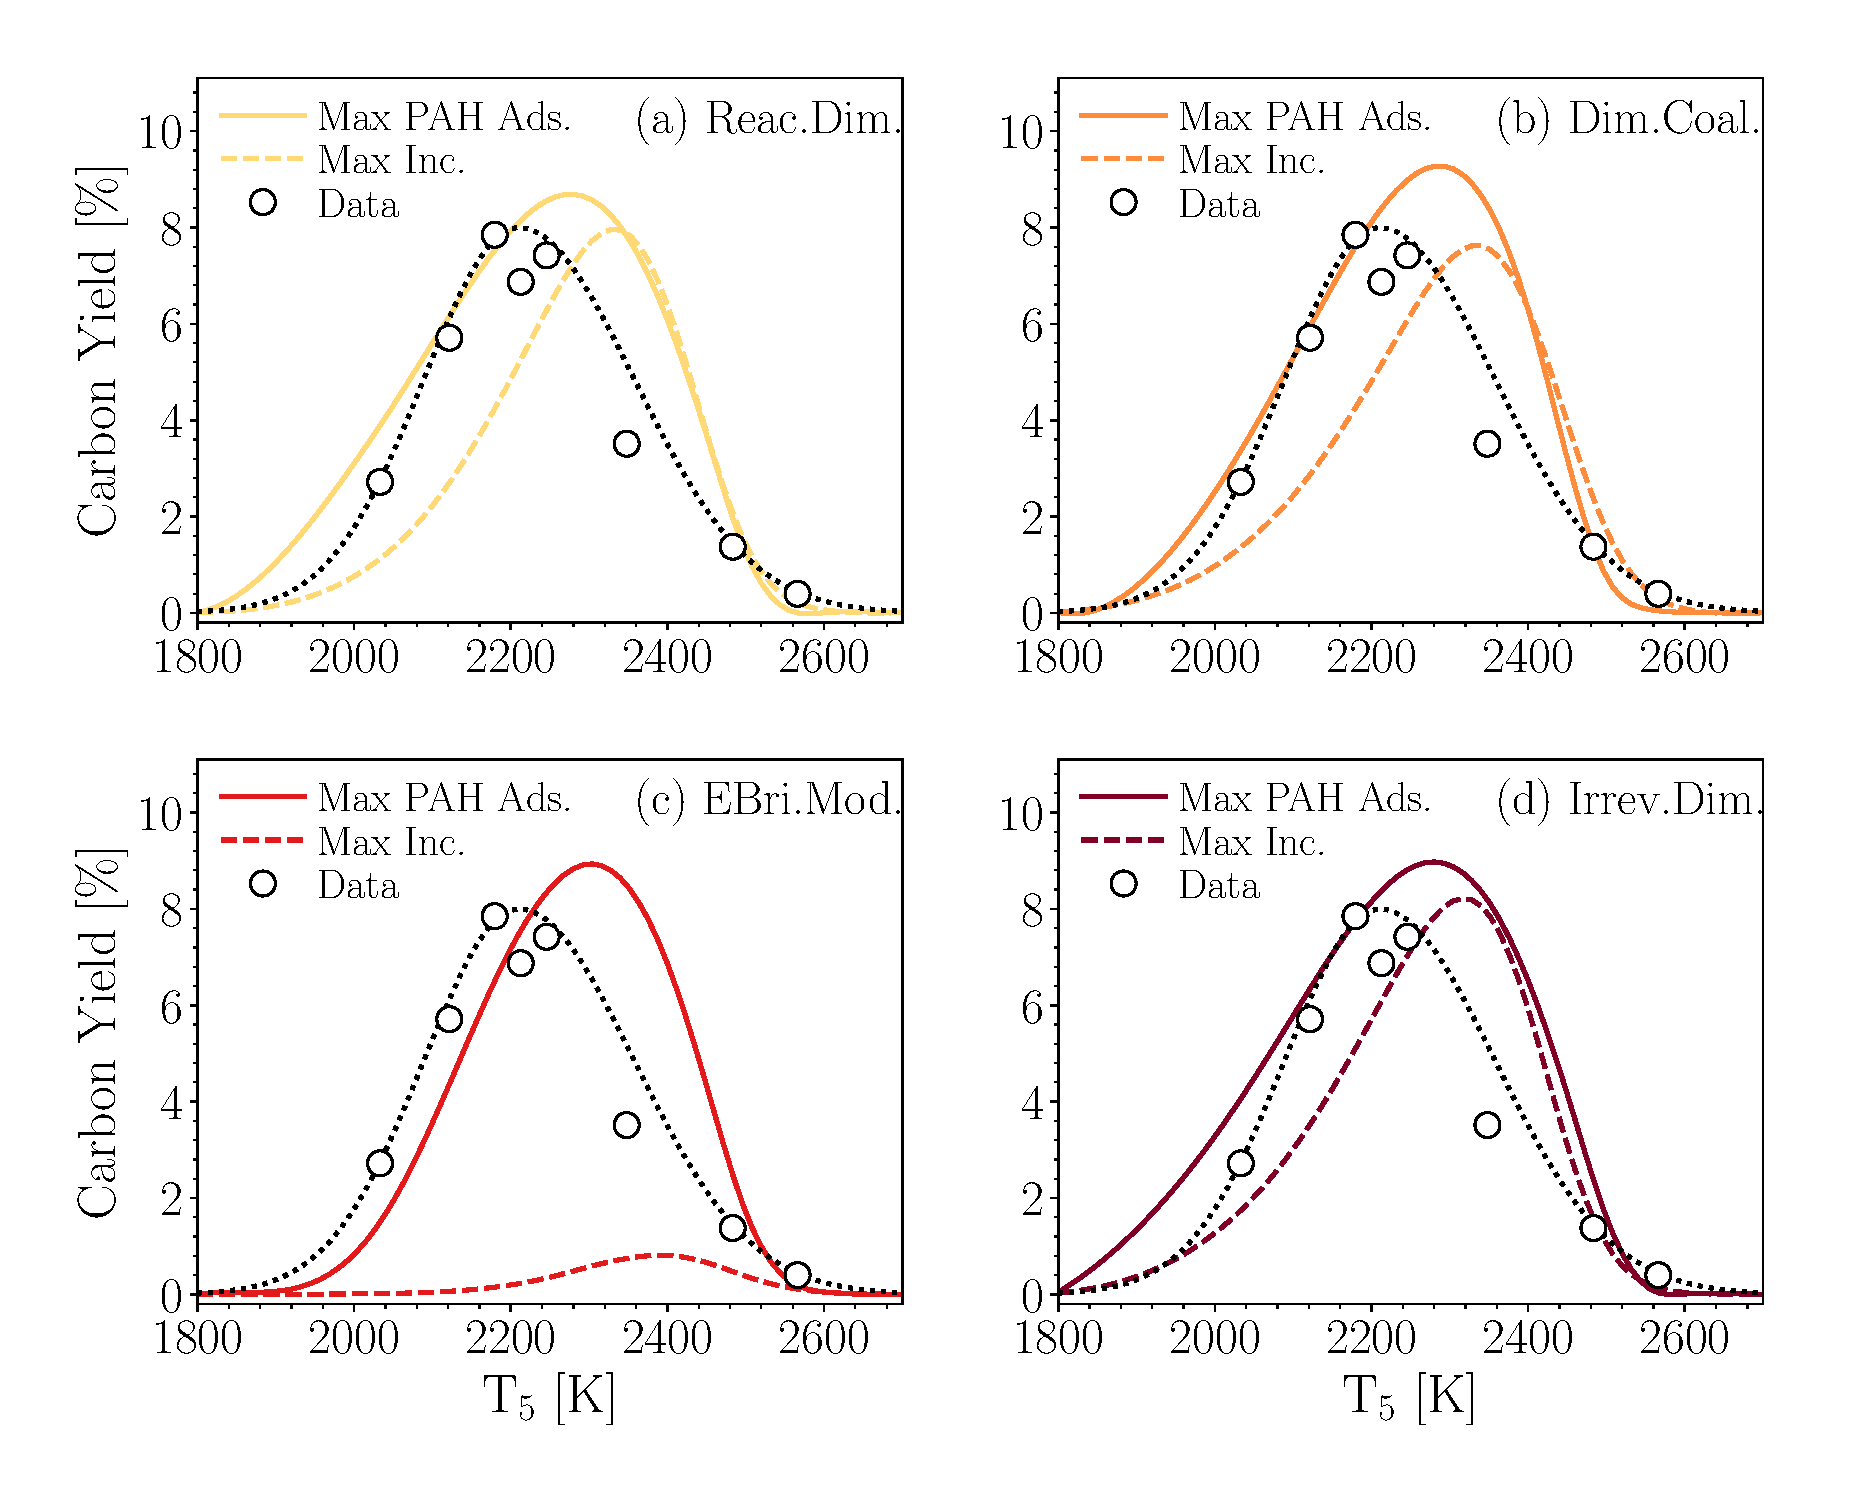
\includegraphics[width=0.8\textwidth]{Figures/Results/Shocktube/Agafonov2016_cvr/carbon_yield_maxincads.pdf}};
		\draw (-3.18, -0.9) node {\scriptsize{\cite{agafonov2016unified}}};
		\draw (2.46, -0.9) node {\scriptsize{\cite{agafonov2016unified}}};
		\draw (-3.18, 3.55) node {\scriptsize{\cite{agafonov2016unified}}};
		\draw (2.46, 3.55) node {\scriptsize{\cite{agafonov2016unified}}};
	\end{tikzpicture}
	\caption{The comparison of soot carbon yield at t=1.5 ms when maximum inception and PAH adsorption were applied to minimized the prediction  error compared to measurements~\citep{agafonov2016unified} for 5\% (a) and 10\%~$\mathrm{CH_4}$ (b) in Ar obtained using Caltech mechanism and different inception models.}
	\label{fig:shockagof_yield_maxincads_cvr} 
\end{figure}

\begin{figure}[H]
	\centering
	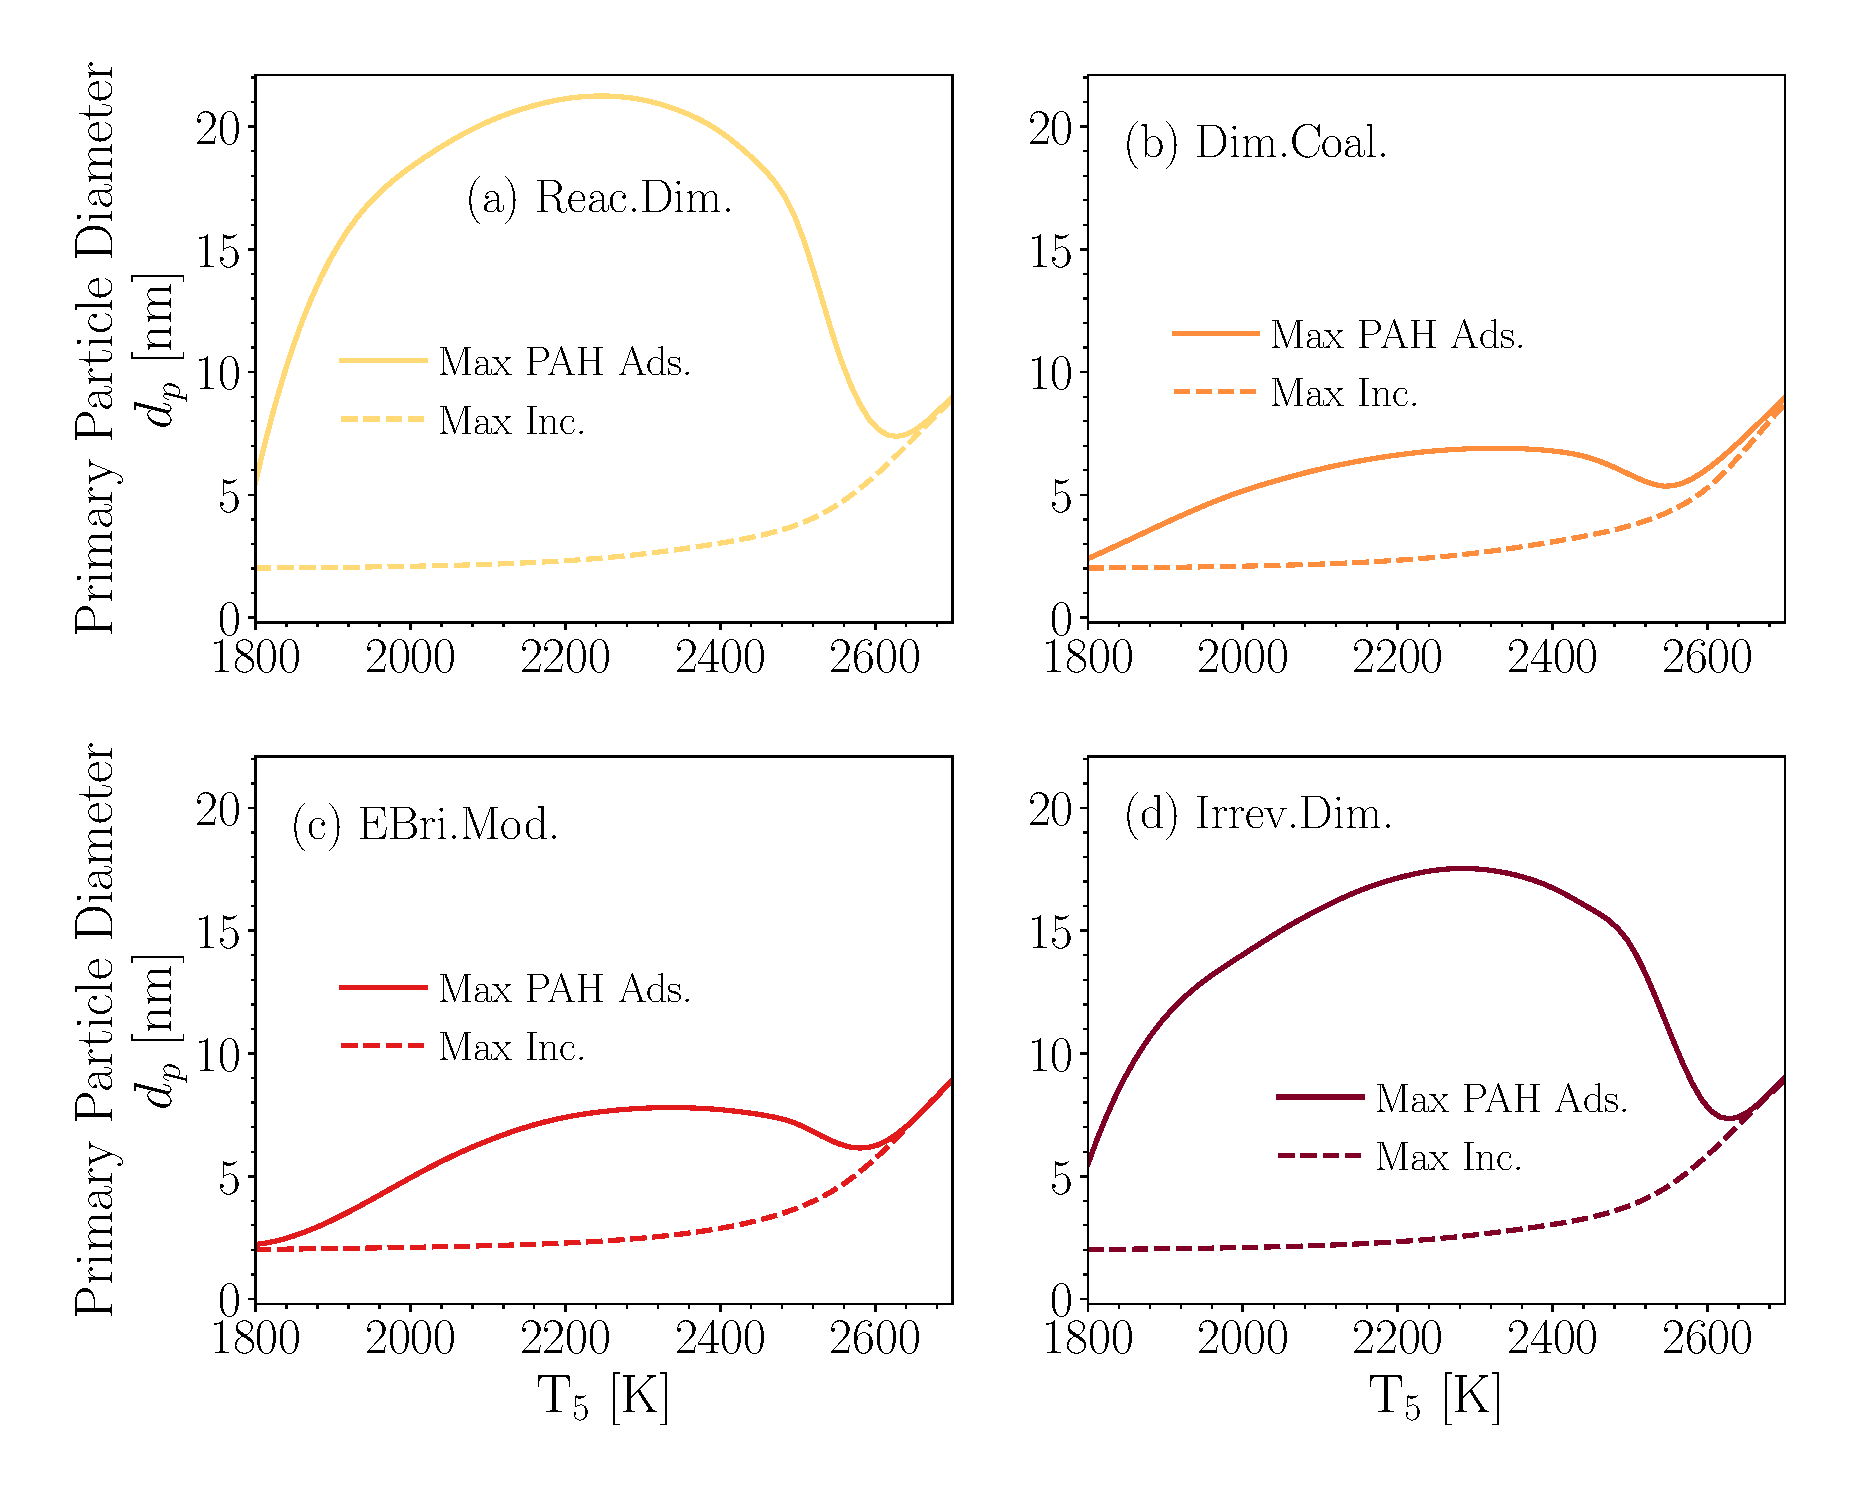
\includegraphics[width=0.8\textwidth]{Figures/Results/Shocktube/Agafonov2016_cvr/d_p_maxincads.pdf}
	\caption{The comparison of mean primary particle, $d_p$ at t=1.5 ms when maximum inception and PAH adsorption were applied to minimized the prediction  error compared to measurements~\citep{agafonov2016unified} for 5\% (a) and 10\%~$\mathrm{CH_4}$ (b) in Ar obtained using Caltech mechanism and different inception models.}
	\label{fig:shockagof_dp_maxincads_cvr} 
\end{figure}